\section{Normal Probability Table}
\label{normalProbabilityTable}

A \term{normal probability table} may be used to
find percentiles of a normal distribution using a Z-score,
or vice-versa.
Such a table lists Z-scores and the corresponding percentiles.
An abbreviated probability table is provided in
Figure~\ref{zTableShort} that we'll use for the examples
in this appendix.
A~full table may be found on page~\pageref{normTableSide1}.

\begin{figure}[h]
\centering
\begin{tabular}{c | rrrrr | rrrrr |}
  \cline{2-11}
&&&& \multicolumn{4}{c}{Second decimal place of $Z$} &&& \\
  \cline{2-11}
$Z$ & \highlightT{0.00} & 0.01 & 0.02 & 0.03 &
    \highlightO{0.04} & 0.05 & 0.06 & 0.07 & 0.08 & 0.09 \\
  \hline
  \hline
0.0 & \footnotesize{0.5000} & \footnotesize{0.5040} & \footnotesize{0.5080} & \footnotesize{0.5120} & \footnotesize{0.5160} & \footnotesize{0.5199} & \footnotesize{0.5239} & \footnotesize{0.5279} & \footnotesize{0.5319} & \footnotesize{0.5359} \\
  0.1 & \footnotesize{0.5398} & \footnotesize{0.5438} & \footnotesize{0.5478} & \footnotesize{0.5517} & \footnotesize{0.5557} & \footnotesize{0.5596} & \footnotesize{0.5636} & \footnotesize{0.5675} & \footnotesize{0.5714} & \footnotesize{0.5753} \\
  0.2 & \footnotesize{0.5793} & \footnotesize{0.5832} & \footnotesize{0.5871} & \footnotesize{0.5910} & \footnotesize{0.5948} & \footnotesize{0.5987} & \footnotesize{0.6026} & \footnotesize{0.6064} & \footnotesize{0.6103} & \footnotesize{0.6141} \\
%  May comment out 0.0-0.2 to make extra space. Then insert the following line:
%  $\vdots$ &   $\vdots$ &   $\vdots$ &   $\vdots$ &   $\vdots$ &   $\vdots$ &   $\vdots$ &   $\vdots$ &   $\vdots$ &   $\vdots$ &   $\vdots$ \\
  0.3 & \footnotesize{0.6179} & \footnotesize{0.6217} & \footnotesize{0.6255} & \footnotesize{0.6293} & \footnotesize{0.6331} & \footnotesize{0.6368} & \footnotesize{0.6406} & \footnotesize{0.6443} & \footnotesize{0.6480} & \footnotesize{0.6517} \\
  0.4 & \footnotesize{0.6554} & \footnotesize{0.6591} & \footnotesize{0.6628} & \footnotesize{0.6664} & \footnotesize{0.6700} & \footnotesize{0.6736} & \footnotesize{0.6772} & \footnotesize{0.6808} & \footnotesize{0.6844} & \footnotesize{0.6879} \\
  \hline
  0.5 & \footnotesize{0.6915} & \footnotesize{0.6950} & \footnotesize{0.6985} & \footnotesize{0.7019} & \footnotesize{0.7054} & \footnotesize{0.7088} & \footnotesize{0.7123} & \footnotesize{0.7157} & \footnotesize{0.7190} & \footnotesize{0.7224} \\
  0.6 & \footnotesize{0.7257} & \footnotesize{0.7291} & \footnotesize{0.7324} & \footnotesize{0.7357} & \footnotesize{0.7389} & \footnotesize{0.7422} & \footnotesize{0.7454} & \footnotesize{0.7486} & \footnotesize{0.7517} & \footnotesize{0.7549} \\
  0.7 & \footnotesize{0.7580} & \footnotesize{0.7611} & \footnotesize{0.7642} & \footnotesize{0.7673} & \footnotesize{0.7704} & \footnotesize{0.7734} & \footnotesize{0.7764} & \footnotesize{0.7794} & \footnotesize{0.7823} & \footnotesize{0.7852} \\
\highlightO{0.8} & \footnotesize{0.7881} & \footnotesize{0.7910} & \footnotesize{0.7939} & \footnotesize{0.7967} & \highlightO{\footnotesize{0.7995}} & \footnotesize{0.8023} & \footnotesize{0.8051} & \footnotesize{0.8078} & \footnotesize{0.8106} & \footnotesize{0.8133} \\
  0.9 & \footnotesize{0.8159} & \footnotesize{0.8186} & \footnotesize{0.8212} & \footnotesize{0.8238} & \footnotesize{0.8264} & \footnotesize{0.8289} & \footnotesize{0.8315} & \footnotesize{0.8340} & \footnotesize{0.8365} & \footnotesize{0.8389} \\
  \hline
  \hline
  \highlightT{1.0} & \highlightT{\footnotesize{0.8413}}
    & \footnotesize{0.8438} & \footnotesize{0.8461} & \footnotesize{0.8485} & \footnotesize{0.8508} & \footnotesize{0.8531} & \footnotesize{0.8554} & \footnotesize{0.8577} & \footnotesize{0.8599} & \footnotesize{0.8621} \\
  1.1 & \footnotesize{0.8643} & \footnotesize{0.8665} & \footnotesize{0.8686} & \footnotesize{0.8708} & \footnotesize{0.8729} & \footnotesize{0.8749} & \footnotesize{0.8770} & \footnotesize{0.8790} & \footnotesize{0.8810} & \footnotesize{0.8830} \\
  $\vdots$ &   $\vdots$ &   $\vdots$ &   $\vdots$ &
      $\vdots$ &   $\vdots$ &   $\vdots$ &   $\vdots$ &
      $\vdots$ &   $\vdots$ &   $\vdots$ \\
   \hline
\end{tabular}
\caption{A section of the normal probability table.
    The percentile for a normal random variable with $Z=1.00$
    has been \highlightT{highlighted}, and the percentile
    closest to 0.8000 has also been \highlightO{highlighted}.}
\label{zTableShort}
\end{figure}

When using a normal probability table to find a percentile
for $Z$ (rounded to two decimals),
identify the proper row in the normal probability
table up through the first decimal, and then determine the
column representing the second decimal value.
The intersection of this row and column is the percentile
of the observation.
For instance, the percentile of $Z = 0.45$ is shown in row
$0.4$ and column $0.05$ in Figure~\ref{zTableShort}:
0.6736, or the $67.36^{th}$ percentile.

\begin{figure}[h]
  \centering
  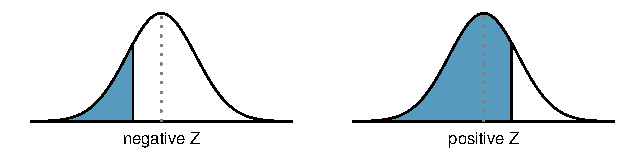
\includegraphics[width=0.8\textwidth]
      {ch_distributions/figures/normalTails/normalTails}
  \caption{The area to the left of $Z$ represents the
      percentile of the observation.}
\end{figure}

\begin{examplewrap}
\begin{nexample}{
    SAT scores follow a normal distribution, $N(1100, 200)$.
    Ann earned a score of 1300 on her SAT with
    a corresponding Z-score of $Z = 1$.
    She would like to know what percentile she falls in among
    all SAT test-takers.}
  Ann's \term{percentile} is the percentage of people who
  earned a lower SAT score than her.
  We shade the area representing those individuals in the
  following graph:
  \begin{center}
  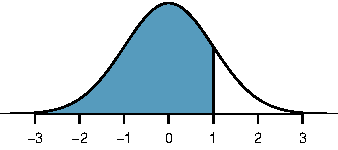
\includegraphics[width=0.45\textwidth]
      {ch_distributions/figures/satBelow1300/satBelow1300}
  \end{center}
  The total area under the normal curve is always equal to~1,
  and the proportion of people who scored below Ann on the SAT
  is equal to the \emph{area} shaded in the graph.
  We find this area by looking in row $1.0$ and column $0.00$
  in the normal probability table:~0.8413.
  In other words, Ann is in the $84^{th}$ percentile of
  SAT takers.
\end{nexample}
\end{examplewrap}

\begin{examplewrap}
\begin{nexample}{How do we find an upper tail area?}
  The normal probability table \emph{always} gives the area
  to the left.
  This means that if we want the area to the right,
  we first find the lower tail and then subtract it from~1.
  For instance, 84.13\% of SAT takers scored below Ann,
  which means 15.87\% of test takers scored higher than Ann.
\end{nexample}
\end{examplewrap}

We can also find the Z-score associated with a percentile.
For example, to identify $Z$ for the $80^{th}$ percentile,
we look for the value closest to 0.8000 in the middle portion
of the table: 0.7995.
We determine the Z-score for the $80^{th}$ percentile by
combining the row and column Z values: 0.84.

\begin{examplewrap}
\begin{nexample}{Find the SAT score for the $80^{th}$ percentile.}
  We look for the are to the value in the table closest to 0.8000.
  The closest value is 0.7995, which corresponds to $Z = 0.84$,
  where 0.8 comes from the row value and 0.04 comes from the
  column value.
  Next, we set up the equation for the Z-score and the unknown
  value $x$ as follows, and then we solve for $x$:
  \begin{align*}
  Z = 0.84 = \frac{x - 1100}{200}
  \quad\to\quad x = 1268
  \end{align*}
  The College Board scales scores to increments of 10,
  so the $80^{th}$ percentile is 1270.
  (Reporting 1268 would have been perfectly okay for our purposes.)
\end{nexample}
\end{examplewrap}

%\noindent%
%Remember: to find the area to the right, calculate 1 minus the area to the left.\vspace{1mm}
%\begin{center}
%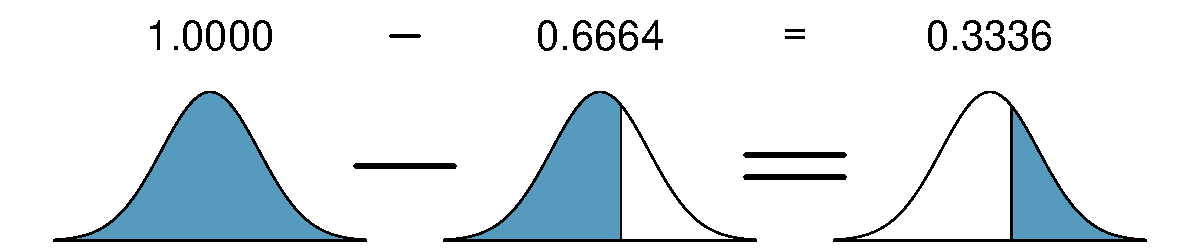
\includegraphics[width=0.55\textwidth]{extraTeX/tables/figures/normalTails/subtractingArea/subtractingArea}\vspace{3mm}
%\end{center}
For additional details about working with the normal distribution and the normal probability table, see Section~\ref{normalDist}, which starts on page~\pageref{normalDist}.

\begin{table}[p]
\begin{center}{\small
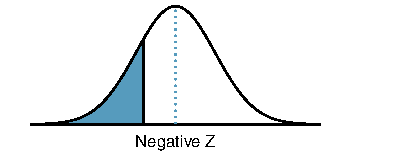
\includegraphics[width=75mm]{extraTeX/tables/figures/normalTails/normalTailLeft} \vspace{2mm} \\
\begin{tabular}{| rrrrr | rrrrr | c}
  \cline{1-10}
&&& \multicolumn{4}{c}{Second decimal place of $Z$} &&& \\
  \cline{1-10}
0.09 &  0.08 &  0.07 &  0.06 &  0.05 &  0.04 &  0.03 &  0.02 &  0.01 &  0.00 & $Z$  \\
  \hline
  \hline
\footnotesize{0.0002} & \footnotesize{0.0003} & \footnotesize{0.0003} & \footnotesize{0.0003} & \footnotesize{0.0003} & \footnotesize{0.0003} & \footnotesize{0.0003} & \footnotesize{0.0003} & \footnotesize{0.0003} & \footnotesize{0.0003} & $-3.4$ \\
  \footnotesize{0.0003} & \footnotesize{0.0004} & \footnotesize{0.0004} & \footnotesize{0.0004} & \footnotesize{0.0004} & \footnotesize{0.0004} & \footnotesize{0.0004} & \footnotesize{0.0005} & \footnotesize{0.0005} & \footnotesize{0.0005} & $-3.3$ \\
  \footnotesize{0.0005} & \footnotesize{0.0005} & \footnotesize{0.0005} & \footnotesize{0.0006} & \footnotesize{0.0006} & \footnotesize{0.0006} & \footnotesize{0.0006} & \footnotesize{0.0006} & \footnotesize{0.0007} & \footnotesize{0.0007} & $-3.2$ \\
  \footnotesize{0.0007} & \footnotesize{0.0007} & \footnotesize{0.0008} & \footnotesize{0.0008} & \footnotesize{0.0008} & \footnotesize{0.0008} & \footnotesize{0.0009} & \footnotesize{0.0009} & \footnotesize{0.0009} & \footnotesize{0.0010} & $-3.1$ \\
  \footnotesize{0.0010} & \footnotesize{0.0010} & \footnotesize{0.0011} & \footnotesize{0.0011} & \footnotesize{0.0011} & \footnotesize{0.0012} & \footnotesize{0.0012} & \footnotesize{0.0013} & \footnotesize{0.0013} & \footnotesize{0.0013} & $-3.0$ \\
    \hline
    \hline
  \footnotesize{0.0014} & \footnotesize{0.0014} & \footnotesize{0.0015} & \footnotesize{0.0015} & \footnotesize{0.0016} & \footnotesize{0.0016} & \footnotesize{0.0017} & \footnotesize{0.0018} & \footnotesize{0.0018} & \footnotesize{0.0019} & $-2.9$ \\
  \footnotesize{0.0019} & \footnotesize{0.0020} & \footnotesize{0.0021} & \footnotesize{0.0021} & \footnotesize{0.0022} & \footnotesize{0.0023} & \footnotesize{0.0023} & \footnotesize{0.0024} & \footnotesize{0.0025} & \footnotesize{0.0026} & $-2.8$ \\
  \footnotesize{0.0026} & \footnotesize{0.0027} & \footnotesize{0.0028} & \footnotesize{0.0029} & \footnotesize{0.0030} & \footnotesize{0.0031} & \footnotesize{0.0032} & \footnotesize{0.0033} & \footnotesize{0.0034} & \footnotesize{0.0035} & $-2.7$ \\
  \footnotesize{0.0036} & \footnotesize{0.0037} & \footnotesize{0.0038} & \footnotesize{0.0039} & \footnotesize{0.0040} & \footnotesize{0.0041} & \footnotesize{0.0043} & \footnotesize{0.0044} & \footnotesize{0.0045} & \footnotesize{0.0047} & $-2.6$ \\
  \footnotesize{0.0048} & \footnotesize{0.0049} & \footnotesize{0.0051} & \footnotesize{0.0052} & \footnotesize{0.0054} & \footnotesize{0.0055} & \footnotesize{0.0057} & \footnotesize{0.0059} & \footnotesize{0.0060} & \footnotesize{0.0062} & $-2.5$ \\
    \hline
  \footnotesize{0.0064} & \footnotesize{0.0066} & \footnotesize{0.0068} & \footnotesize{0.0069} & \footnotesize{0.0071} & \footnotesize{0.0073} & \footnotesize{0.0075} & \footnotesize{0.0078} & \footnotesize{0.0080} & \footnotesize{0.0082} & $-2.4$ \\
  \footnotesize{0.0084} & \footnotesize{0.0087} & \footnotesize{0.0089} & \footnotesize{0.0091} & \footnotesize{0.0094} & \footnotesize{0.0096} & \footnotesize{0.0099} & \footnotesize{0.0102} & \footnotesize{0.0104} & \footnotesize{0.0107} & $-2.3$ \\
  \footnotesize{0.0110} & \footnotesize{0.0113} & \footnotesize{0.0116} & \footnotesize{0.0119} & \footnotesize{0.0122} & \footnotesize{0.0125} & \footnotesize{0.0129} & \footnotesize{0.0132} & \footnotesize{0.0136} & \footnotesize{0.0139} & $-2.2$ \\
  \footnotesize{0.0143} & \footnotesize{0.0146} & \footnotesize{0.0150} & \footnotesize{0.0154} & \footnotesize{0.0158} & \footnotesize{0.0162} & \footnotesize{0.0166} & \footnotesize{0.0170} & \footnotesize{0.0174} & \footnotesize{0.0179} & $-2.1$ \\
  \footnotesize{0.0183} & \footnotesize{0.0188} & \footnotesize{0.0192} & \footnotesize{0.0197} & \footnotesize{0.0202} & \footnotesize{0.0207} & \footnotesize{0.0212} & \footnotesize{0.0217} & \footnotesize{0.0222} & \footnotesize{0.0228} & $-2.0$ \\
    \hline
    \hline
  \footnotesize{0.0233} & \footnotesize{0.0239} & \footnotesize{0.0244} & \footnotesize{0.0250} & \footnotesize{0.0256} & \footnotesize{0.0262} & \footnotesize{0.0268} & \footnotesize{0.0274} & \footnotesize{0.0281} & \footnotesize{0.0287} & $-1.9$ \\
  \footnotesize{0.0294} & \footnotesize{0.0301} & \footnotesize{0.0307} & \footnotesize{0.0314} & \footnotesize{0.0322} & \footnotesize{0.0329} & \footnotesize{0.0336} & \footnotesize{0.0344} & \footnotesize{0.0351} & \footnotesize{0.0359} & $-1.8$ \\
  \footnotesize{0.0367} & \footnotesize{0.0375} & \footnotesize{0.0384} & \footnotesize{0.0392} & \footnotesize{0.0401} & \footnotesize{0.0409} & \footnotesize{0.0418} & \footnotesize{0.0427} & \footnotesize{0.0436} & \footnotesize{0.0446} & $-1.7$ \\
  \footnotesize{0.0455} & \footnotesize{0.0465} & \footnotesize{0.0475} & \footnotesize{0.0485} & \footnotesize{0.0495} & \footnotesize{0.0505} & \footnotesize{0.0516} & \footnotesize{0.0526} & \footnotesize{0.0537} & \footnotesize{0.0548} & $-1.6$ \\
  \footnotesize{0.0559} & \footnotesize{0.0571} & \footnotesize{0.0582} & \footnotesize{0.0594} & \footnotesize{0.0606} & \footnotesize{0.0618} & \footnotesize{0.0630} & \footnotesize{0.0643} & \footnotesize{0.0655} & \footnotesize{0.0668} & $-1.5$ \\
    \hline
  \footnotesize{0.0681} & \footnotesize{0.0694} & \footnotesize{0.0708} & \footnotesize{0.0721} & \footnotesize{0.0735} & \footnotesize{0.0749} & \footnotesize{0.0764} & \footnotesize{0.0778} & \footnotesize{0.0793} & \footnotesize{0.0808} & $-1.4$ \\
  \footnotesize{0.0823} & \footnotesize{0.0838} & \footnotesize{0.0853} & \footnotesize{0.0869} & \footnotesize{0.0885} & \footnotesize{0.0901} & \footnotesize{0.0918} & \footnotesize{0.0934} & \footnotesize{0.0951} & \footnotesize{0.0968} & $-1.3$ \\
  \footnotesize{0.0985} & \footnotesize{0.1003} & \footnotesize{0.1020} & \footnotesize{0.1038} & \footnotesize{0.1056} & \footnotesize{0.1075} & \footnotesize{0.1093} & \footnotesize{0.1112} & \footnotesize{0.1131} & \footnotesize{0.1151} & $-1.2$ \\
  \footnotesize{0.1170} & \footnotesize{0.1190} & \footnotesize{0.1210} & \footnotesize{0.1230} & \footnotesize{0.1251} & \footnotesize{0.1271} & \footnotesize{0.1292} & \footnotesize{0.1314} & \footnotesize{0.1335} & \footnotesize{0.1357} & $-1.1$ \\
  \footnotesize{0.1379} & \footnotesize{0.1401} & \footnotesize{0.1423} & \footnotesize{0.1446} & \footnotesize{0.1469} & \footnotesize{0.1492} & \footnotesize{0.1515} & \footnotesize{0.1539} & \footnotesize{0.1562} & \footnotesize{0.1587} & $-1.0$ \\
    \hline
    \hline
  \footnotesize{0.1611} & \footnotesize{0.1635} & \footnotesize{0.1660} & \footnotesize{0.1685} & \footnotesize{0.1711} & \footnotesize{0.1736} & \footnotesize{0.1762} & \footnotesize{0.1788} & \footnotesize{0.1814} & \footnotesize{0.1841} & $-0.9$ \\
  \footnotesize{0.1867} & \footnotesize{0.1894} & \footnotesize{0.1922} & \footnotesize{0.1949} & \footnotesize{0.1977} & \footnotesize{0.2005} & \footnotesize{0.2033} & \footnotesize{0.2061} & \footnotesize{0.2090} & \footnotesize{0.2119} & $-0.8$ \\
  \footnotesize{0.2148} & \footnotesize{0.2177} & \footnotesize{0.2206} & \footnotesize{0.2236} & \footnotesize{0.2266} & \footnotesize{0.2296} & \footnotesize{0.2327} & \footnotesize{0.2358} & \footnotesize{0.2389} & \footnotesize{0.2420} & $-0.7$ \\
  \footnotesize{0.2451} & \footnotesize{0.2483} & \footnotesize{0.2514} & \footnotesize{0.2546} & \footnotesize{0.2578} & \footnotesize{0.2611} & \footnotesize{0.2643} & \footnotesize{0.2676} & \footnotesize{0.2709} & \footnotesize{0.2743} & $-0.6$ \\
  \footnotesize{0.2776} & \footnotesize{0.2810} & \footnotesize{0.2843} & \footnotesize{0.2877} & \footnotesize{0.2912} & \footnotesize{0.2946} & \footnotesize{0.2981} & \footnotesize{0.3015} & \footnotesize{0.3050} & \footnotesize{0.3085} & $-0.5$ \\
    \hline
  \footnotesize{0.3121} & \footnotesize{0.3156} & \footnotesize{0.3192} & \footnotesize{0.3228} & \footnotesize{0.3264} & \footnotesize{0.3300} & \footnotesize{0.3336} & \footnotesize{0.3372} & \footnotesize{0.3409} & \footnotesize{0.3446} & $-0.4$ \\
  \footnotesize{0.3483} & \footnotesize{0.3520} & \footnotesize{0.3557} & \footnotesize{0.3594} & \footnotesize{0.3632} & \footnotesize{0.3669} & \footnotesize{0.3707} & \footnotesize{0.3745} & \footnotesize{0.3783} & \footnotesize{0.3821} & $-0.3$ \\
  \footnotesize{0.3859} & \footnotesize{0.3897} & \footnotesize{0.3936} & \footnotesize{0.3974} & \footnotesize{0.4013} & \footnotesize{0.4052} & \footnotesize{0.4090} & \footnotesize{0.4129} & \footnotesize{0.4168} & \footnotesize{0.4207} & $-0.2$ \\
  \footnotesize{0.4247} & \footnotesize{0.4286} & \footnotesize{0.4325} & \footnotesize{0.4364} & \footnotesize{0.4404} & \footnotesize{0.4443} & \footnotesize{0.4483} & \footnotesize{0.4522} & \footnotesize{0.4562} & \footnotesize{0.4602} & $-0.1$ \\
  \footnotesize{0.4641} & \footnotesize{0.4681} & \footnotesize{0.4721} & \footnotesize{0.4761} & \footnotesize{0.4801} & \footnotesize{0.4840} & \footnotesize{0.4880} & \footnotesize{0.4920} & \footnotesize{0.4960} & \footnotesize{0.5000} & $-0.0$ \\
    \hline
\multicolumn{11}{l}{{\normalsize$^*$For $Z \leq -3.50$, the probability is less than or equal to $0.0002$.}}
\end{tabular}}
\label{normTableSide1}
\end{center}
\end{table}

\begin{table}[p]
\begin{center}{\small
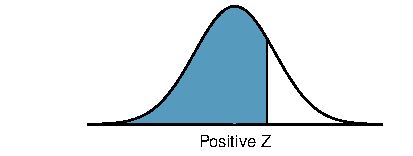
\includegraphics[width=75mm]{extraTeX/tables/figures/normalTails/normalTailRight} \vspace{2mm} \\
\begin{tabular}{c | rrrrr | rrrrr |}
  \cline{2-11}
&&&& \multicolumn{4}{c}{Second decimal place of $Z$} &&& \\
  \cline{2-11}
$Z$ & 0.00 & 0.01 & 0.02 & 0.03 & 0.04 & 0.05 & 0.06 & 0.07 & 0.08 & 0.09 \\
  \hline
  \hline
0.0 & \footnotesize{0.5000} & \footnotesize{0.5040} & \footnotesize{0.5080} & \footnotesize{0.5120} & \footnotesize{0.5160} & \footnotesize{0.5199} & \footnotesize{0.5239} & \footnotesize{0.5279} & \footnotesize{0.5319} & \footnotesize{0.5359} \\
  0.1 & \footnotesize{0.5398} & \footnotesize{0.5438} & \footnotesize{0.5478} & \footnotesize{0.5517} & \footnotesize{0.5557} & \footnotesize{0.5596} & \footnotesize{0.5636} & \footnotesize{0.5675} & \footnotesize{0.5714} & \footnotesize{0.5753} \\
  0.2 & \footnotesize{0.5793} & \footnotesize{0.5832} & \footnotesize{0.5871} & \footnotesize{0.5910} & \footnotesize{0.5948} & \footnotesize{0.5987} & \footnotesize{0.6026} & \footnotesize{0.6064} & \footnotesize{0.6103} & \footnotesize{0.6141} \\
  0.3 & \footnotesize{0.6179} & \footnotesize{0.6217} & \footnotesize{0.6255} & \footnotesize{0.6293} & \footnotesize{0.6331} & \footnotesize{0.6368} & \footnotesize{0.6406} & \footnotesize{0.6443} & \footnotesize{0.6480} & \footnotesize{0.6517} \\
  0.4 & \footnotesize{0.6554} & \footnotesize{0.6591} & \footnotesize{0.6628} & \footnotesize{0.6664} & \footnotesize{0.6700} & \footnotesize{0.6736} & \footnotesize{0.6772} & \footnotesize{0.6808} & \footnotesize{0.6844} & \footnotesize{0.6879} \\
  \hline
  0.5 & \footnotesize{0.6915} & \footnotesize{0.6950} & \footnotesize{0.6985} & \footnotesize{0.7019} & \footnotesize{0.7054} & \footnotesize{0.7088} & \footnotesize{0.7123} & \footnotesize{0.7157} & \footnotesize{0.7190} & \footnotesize{0.7224} \\
  0.6 & \footnotesize{0.7257} & \footnotesize{0.7291} & \footnotesize{0.7324} & \footnotesize{0.7357} & \footnotesize{0.7389} & \footnotesize{0.7422} & \footnotesize{0.7454} & \footnotesize{0.7486} & \footnotesize{0.7517} & \footnotesize{0.7549} \\
  0.7 & \footnotesize{0.7580} & \footnotesize{0.7611} & \footnotesize{0.7642} & \footnotesize{0.7673} & \footnotesize{0.7704} & \footnotesize{0.7734} & \footnotesize{0.7764} & \footnotesize{0.7794} & \footnotesize{0.7823} & \footnotesize{0.7852} \\
  0.8 & \footnotesize{0.7881} & \footnotesize{0.7910} & \footnotesize{0.7939} & \footnotesize{0.7967} & \footnotesize{0.7995} & \footnotesize{0.8023} & \footnotesize{0.8051} & \footnotesize{0.8078} & \footnotesize{0.8106} & \footnotesize{0.8133} \\
  0.9 & \footnotesize{0.8159} & \footnotesize{0.8186} & \footnotesize{0.8212} & \footnotesize{0.8238} & \footnotesize{0.8264} & \footnotesize{0.8289} & \footnotesize{0.8315} & \footnotesize{0.8340} & \footnotesize{0.8365} & \footnotesize{0.8389} \\
  \hline
  \hline
  1.0 & \footnotesize{0.8413} & \footnotesize{0.8438} & \footnotesize{0.8461} & \footnotesize{0.8485} & \footnotesize{0.8508} & \footnotesize{0.8531} & \footnotesize{0.8554} & \footnotesize{0.8577} & \footnotesize{0.8599} & \footnotesize{0.8621} \\
  1.1 & \footnotesize{0.8643} & \footnotesize{0.8665} & \footnotesize{0.8686} & \footnotesize{0.8708} & \footnotesize{0.8729} & \footnotesize{0.8749} & \footnotesize{0.8770} & \footnotesize{0.8790} & \footnotesize{0.8810} & \footnotesize{0.8830} \\
  1.2 & \footnotesize{0.8849} & \footnotesize{0.8869} & \footnotesize{0.8888} & \footnotesize{0.8907} & \footnotesize{0.8925} & \footnotesize{0.8944} & \footnotesize{0.8962} & \footnotesize{0.8980} & \footnotesize{0.8997} & \footnotesize{0.9015} \\
  1.3 & \footnotesize{0.9032} & \footnotesize{0.9049} & \footnotesize{0.9066} & \footnotesize{0.9082} & \footnotesize{0.9099} & \footnotesize{0.9115} & \footnotesize{0.9131} & \footnotesize{0.9147} & \footnotesize{0.9162} & \footnotesize{0.9177} \\
  1.4 & \footnotesize{0.9192} & \footnotesize{0.9207} & \footnotesize{0.9222} & \footnotesize{0.9236} & \footnotesize{0.9251} & \footnotesize{0.9265} & \footnotesize{0.9279} & \footnotesize{0.9292} & \footnotesize{0.9306} & \footnotesize{0.9319} \\
  \hline
  1.5 & \footnotesize{0.9332} & \footnotesize{0.9345} & \footnotesize{0.9357} & \footnotesize{0.9370} & \footnotesize{0.9382} & \footnotesize{0.9394} & \footnotesize{0.9406} & \footnotesize{0.9418} & \footnotesize{0.9429} & \footnotesize{0.9441} \\
  1.6 & \footnotesize{0.9452} & \footnotesize{0.9463} & \footnotesize{0.9474} & \footnotesize{0.9484} & \footnotesize{0.9495} & \footnotesize{0.9505} & \footnotesize{0.9515} & \footnotesize{0.9525} & \footnotesize{0.9535} & \footnotesize{0.9545} \\
  1.7 & \footnotesize{0.9554} & \footnotesize{0.9564} & \footnotesize{0.9573} & \footnotesize{0.9582} & \footnotesize{0.9591} & \footnotesize{0.9599} & \footnotesize{0.9608} & \footnotesize{0.9616} & \footnotesize{0.9625} & \footnotesize{0.9633} \\
  1.8 & \footnotesize{0.9641} & \footnotesize{0.9649} & \footnotesize{0.9656} & \footnotesize{0.9664} & \footnotesize{0.9671} & \footnotesize{0.9678} & \footnotesize{0.9686} & \footnotesize{0.9693} & \footnotesize{0.9699} & \footnotesize{0.9706} \\
  1.9 & \footnotesize{0.9713} & \footnotesize{0.9719} & \footnotesize{0.9726} & \footnotesize{0.9732} & \footnotesize{0.9738} & \footnotesize{0.9744} & \footnotesize{0.9750} & \footnotesize{0.9756} & \footnotesize{0.9761} & \footnotesize{0.9767} \\
  \hline
  \hline
  2.0 & \footnotesize{0.9772} & \footnotesize{0.9778} & \footnotesize{0.9783} & \footnotesize{0.9788} & \footnotesize{0.9793} & \footnotesize{0.9798} & \footnotesize{0.9803} & \footnotesize{0.9808} & \footnotesize{0.9812} & \footnotesize{0.9817} \\
  2.1 & \footnotesize{0.9821} & \footnotesize{0.9826} & \footnotesize{0.9830} & \footnotesize{0.9834} & \footnotesize{0.9838} & \footnotesize{0.9842} & \footnotesize{0.9846} & \footnotesize{0.9850} & \footnotesize{0.9854} & \footnotesize{0.9857} \\
  2.2 & \footnotesize{0.9861} & \footnotesize{0.9864} & \footnotesize{0.9868} & \footnotesize{0.9871} & \footnotesize{0.9875} & \footnotesize{0.9878} & \footnotesize{0.9881} & \footnotesize{0.9884} & \footnotesize{0.9887} & \footnotesize{0.9890} \\
  2.3 & \footnotesize{0.9893} & \footnotesize{0.9896} & \footnotesize{0.9898} & \footnotesize{0.9901} & \footnotesize{0.9904} & \footnotesize{0.9906} & \footnotesize{0.9909} & \footnotesize{0.9911} & \footnotesize{0.9913} & \footnotesize{0.9916} \\
  2.4 & \footnotesize{0.9918} & \footnotesize{0.9920} & \footnotesize{0.9922} & \footnotesize{0.9925} & \footnotesize{0.9927} & \footnotesize{0.9929} & \footnotesize{0.9931} & \footnotesize{0.9932} & \footnotesize{0.9934} & \footnotesize{0.9936} \\
  \hline
  2.5 & \footnotesize{0.9938} & \footnotesize{0.9940} & \footnotesize{0.9941} & \footnotesize{0.9943} & \footnotesize{0.9945} & \footnotesize{0.9946} & \footnotesize{0.9948} & \footnotesize{0.9949} & \footnotesize{0.9951} & \footnotesize{0.9952} \\
  2.6 & \footnotesize{0.9953} & \footnotesize{0.9955} & \footnotesize{0.9956} & \footnotesize{0.9957} & \footnotesize{0.9959} & \footnotesize{0.9960} & \footnotesize{0.9961} & \footnotesize{0.9962} & \footnotesize{0.9963} & \footnotesize{0.9964} \\
  2.7 & \footnotesize{0.9965} & \footnotesize{0.9966} & \footnotesize{0.9967} & \footnotesize{0.9968} & \footnotesize{0.9969} & \footnotesize{0.9970} & \footnotesize{0.9971} & \footnotesize{0.9972} & \footnotesize{0.9973} & \footnotesize{0.9974} \\
  2.8 & \footnotesize{0.9974} & \footnotesize{0.9975} & \footnotesize{0.9976} & \footnotesize{0.9977} & \footnotesize{0.9977} & \footnotesize{0.9978} & \footnotesize{0.9979} & \footnotesize{0.9979} & \footnotesize{0.9980} & \footnotesize{0.9981} \\
  2.9 & \footnotesize{0.9981} & \footnotesize{0.9982} & \footnotesize{0.9982} & \footnotesize{0.9983} & \footnotesize{0.9984} & \footnotesize{0.9984} & \footnotesize{0.9985} & \footnotesize{0.9985} & \footnotesize{0.9986} & \footnotesize{0.9986} \\
  \hline
  \hline
  3.0 & \footnotesize{0.9987} & \footnotesize{0.9987} & \footnotesize{0.9987} & \footnotesize{0.9988} & \footnotesize{0.9988} & \footnotesize{0.9989} & \footnotesize{0.9989} & \footnotesize{0.9989} & \footnotesize{0.9990} & \footnotesize{0.9990} \\
  3.1 & \footnotesize{0.9990} & \footnotesize{0.9991} & \footnotesize{0.9991} & \footnotesize{0.9991} & \footnotesize{0.9992} & \footnotesize{0.9992} & \footnotesize{0.9992} & \footnotesize{0.9992} & \footnotesize{0.9993} & \footnotesize{0.9993} \\
  3.2 & \footnotesize{0.9993} & \footnotesize{0.9993} & \footnotesize{0.9994} & \footnotesize{0.9994} & \footnotesize{0.9994} & \footnotesize{0.9994} & \footnotesize{0.9994} & \footnotesize{0.9995} & \footnotesize{0.9995} & \footnotesize{0.9995} \\
  3.3 & \footnotesize{0.9995} & \footnotesize{0.9995} & \footnotesize{0.9995} & \footnotesize{0.9996} & \footnotesize{0.9996} & \footnotesize{0.9996} & \footnotesize{0.9996} & \footnotesize{0.9996} & \footnotesize{0.9996} & \footnotesize{0.9997} \\
  3.4 & \footnotesize{0.9997} & \footnotesize{0.9997} & \footnotesize{0.9997} & \footnotesize{0.9997} & \footnotesize{0.9997} & \footnotesize{0.9997} & \footnotesize{0.9997} & \footnotesize{0.9997} & \footnotesize{0.9997} & \footnotesize{0.9998} \\
   \hline
\multicolumn{11}{l}{{\normalsize$^*$For $Z \geq 3.50$, the probability is greater than or equal to $0.9998$.}}
\end{tabular}}
\end{center}
\end{table}
